\documentclass[conference]{IEEEtran}
\usepackage{float}

% \IEEEoverridecommandlockouts
% The preceding line is only needed to identify funding in the first footnote. If that is unneeded, please comment it out.
\usepackage{cite}
\usepackage{amsmath,amssymb,amsfonts}
\usepackage{algorithmic}
\usepackage{amsmath}
\usepackage{graphicx}
\usepackage{textcomp}
\usepackage{xcolor}
\def\BibTeX{{\rm B\kern-.05em{\sc i\kern-.025em b}\kern-.08em
    T\kern-.1667em\lower.7ex\hbox{E}\kern-.125emX}}
\begin{document}

\title{Project Report: Interactive Car Game Using Microcontroller\\}

\author{
\centering
\IEEEauthorblockN{1\textsuperscript{st} Mateo Ronflard}
\IEEEauthorblockA{\textit{Computer Engineering} \\
\textit{McGill University} \\
Montreal, Canada \\
mateo.ronflard@mail.mcgill.ca, 260974012}
\vspace{1em}
\IEEEauthorblockN{2\textsuperscript{nd} Elie-Dimitri Abdo}
\IEEEauthorblockA{\textit{Computer Engineering} \\
\textit{McGill University} \\
Montreal, Canada \\
elie-dimitri.abdo@mail.mcgill.ca, 260948346}
\and
\IEEEauthorblockN{3\textsuperscript{rd} Alex Cattani}
\IEEEauthorblockA{\textit{Computer Engineering} \\
\textit{McGill University} \\
Montreal, Canada \\
alex.cattani@mail.mcgill.ca, 260924860}
\vspace{1em}
\IEEEauthorblockN{4\textsuperscript{th} Philippe Olivier Fils}
\IEEEauthorblockA{\textit{Computer Engineering} \\
\textit{McGill University} \\
Montreal, Canada \\
philippe.fils@mail.mcgill.ca, 260989600}
}
\maketitle

\begin{abstract}
This project implements a dynamic and interactive car game on an embedded system, showcasing advanced features such as UART communication for real-time game display, I2C-based tilt control for player interaction, auditory feedback through a DAC and speaker, and a custom operating system for thread management. The primary focus is on tilt control, which leverages accelerometer data to navigate menus and control car movements in the game. The mathematical principles behind tilt calculation, including angle determination and boundary constraints, are detailed. This project highlights the integration of hardware and software to achieve a responsive and engaging gaming experience, demonstrating the capabilities of microcontroller-based systems in real-time applications.
\end{abstract}

\textbf{Keywords:} Embedded systems, UART communication, tilt control, DAC, real-time operating system, interactive gaming, accelerometer, I2C, thread management.

\section{Introduction}
Embedded systems have revolutionized the way we interact with technology, enabling the creation of sophisticated real-time applications with minimal hardware. This project focuses on the design and implementation of an interactive car game using an embedded microcontroller. By leveraging advanced communication protocols, audio-visual feedback mechanisms, and multitasking capabilities, this game demonstrates the potential of embedded systems in delivering engaging user experiences.

The game consists of multiple interconnected features, including real-time game display via UART, tilt-based controls using I2C, auditory feedback through a DAC and speaker, and a custom operating system (OS) for managing threads. These features collectively form a robust system that highlights the importance of integrating software and hardware for high-performance embedded applications.

Tilt-based control is the core feature of this project, offering an innovative way for players to navigate menus and control the car's movement during gameplay. The accelerometer data is processed using mathematical models to calculate the tilt angle and translate it into meaningful actions. This ensures an intuitive and responsive user interaction, bridging the gap between physical movements and in-game actions.

By detailing both the design and implementation, this report aims to showcase not only the technical accomplishments but also the methodologies used to achieve a seamless gaming experience. The project demonstrates the versatility of embedded systems in creating real-time interactive applications, making it a valuable learning experience and a proof of concept for future developments.

\section{Project Features}
\subsection{UART Communication for Game Display}
The game leverages UART communication to print the road layout and car position on a terminal. This feature provides real-time visual feedback of the car's movement relative to the road boundaries. The dynamic display updates continuously as the player interacts with the game, making it easy to monitor gameplay progress. This feature highlights the integration of serial communication protocols to achieve seamless data transfer.

\subsection{Tilt Control Using I2C}
The tilt control feature is central to the game, allowing the player to navigate the car within the game environment and interact with the menu. This functionality is achieved by interfacing an accelerometer with the microcontroller via the I2C protocol. The accelerometer measures the tilt angles of the device, which are used to determine the car's movement and menu selections.

\subsubsection{Mathematics of Tilt-Based Control}
The tilt-based control mechanism utilizes accelerometer data to calculate the car's roll angle and determine its movement along the road. The accelerometer provides three-dimensional data: $a_x$, $a_y$, and $a_z$, representing the acceleration along the $x$, $y$, and $z$ axes, respectively. 

To calculate the roll angle $\phi$ (in degrees), the following steps are performed:
\begin{enumerate}
    \item Compute the magnitude of the horizontal components of acceleration $a_x$ and $a_z$:
    \begin{equation}
    M = \sqrt{a_x^2 + a_z^2}
    \end{equation}
    This magnitude represents the combined horizontal acceleration components and is necessary for determining the roll angle.

    \item Using the calculated magnitude $M$, determine the roll angle $\phi$ using the $\text{atan2}$ function. The $\text{atan2}$ function takes the vertical acceleration $a_y$ and the horizontal magnitude $M$ as arguments:
    \begin{equation}
    \phi = \text{atan2}(a_y, M) \cdot \frac{180}{\pi}
    \end{equation}
    Here, the factor $\frac{180}{\pi} \approx 57.2958$ is used to convert the roll angle from radians to degrees.

    \item The roll angle $\phi$ is then compared to thresholds to determine the car's movement along the road:
\begin{itemize}
    \item If $\phi > 20.0^\circ$ and \texttt{car\_position} $< 6$, update \texttt{car\_position} as: 
    \[
    \texttt{car\_position} \leftarrow \texttt{car\_position} + 1
    \]
    \item If $\phi < -20.0^\circ$ and \texttt{car\_position} $> 0$, update \texttt{car\_position} as: 
    \[
    \texttt{car\_position} \leftarrow \texttt{car\_position} - 1
    \]
\end{itemize}

    These conditions ensure that the car moves left or right based on the tilt of the device while staying within the allowed boundaries of the road.
\end{enumerate}

To ensure thread safety when updating the car's position, the accelerometer data is protected using a mutex. The following steps outline this process:
\begin{enumerate}
    \item The mutex is acquired to prevent concurrent access:
    \begin{equation}
    \text{osMutexWait(accelDataMutex, osWaitForever)}
    \end{equation}

    \item The car's position is updated based on the computed roll angle $\phi$ and the defined thresholds.

    \item The mutex is released after the update:
    \begin{equation}
    \text{osMutexRelease(accelDataMutex)}
    \end{equation}
\end{enumerate}

This approach ensures real-time responsiveness and prevents data corruption caused by simultaneous thread access. By combining precise mathematical computations and robust synchronization mechanisms, the system achieves smooth and accurate tilt-based control for the car.


\subsubsection{Menu Navigation Using Tilt Control and Button}
Tilt control is also used for menu navigation. The accelerometer readings are processed similarly, with predefined tilt ranges mapped to moving up or down in the menu options. To select and option, the user presses the button and this effectively starts the game.

\subsection{Auditory Feedback Using DAC and Speaker}
Auditory feedback is provided through a speaker connected to the microcontroller's DAC. This feature generates sound effects when the car interacts with the game environment, such as collisions, crossing boundaries, or successfully completing a level. The DAC converts digital signals into analog waveforms, driving the speaker to produce sound. This enhances the game’s interactivity by engaging multiple senses.

\subsubsection{Speaker Setup}
The speaker is connected to the DAC output pin on the microcontroller. The DAC is configured to produce varying signal levels to modulate sound pitches and volumes. Key details include:
\begin{itemize}
    \item \textbf{Hardware Connection:} The DAC output is connected to a low-power speaker via a coupling capacitor to filter out DC offsets.
    \item \textbf{Signal Modulation:} The DAC generates waveforms of different frequencies and durations to create distinct sound effects.
    \item \textbf{Volume Control:} By adjusting the amplitude of the generated waveform, the volume can be controlled programmatically.
    \item \textbf{Improved Loudness:} The speaker's volume was optimized by ensuring maximum safe DAC output levels and experimenting with different coupling capacitor values to enhance audio output.
\end{itemize}

\subsubsection{Sound Effects Implementation}
The game features multiple sound effects to enhance player immersion:
\begin{itemize}
    \item \textbf{Collision Alert:} A sharp tone of fixed duration to notify the player of a collision.
    \item \textbf{Boundary Warning:} A short beep when the car attempts to cross the road boundaries.
    \item \textbf{Victory Sound:} A sequence of tones of varying pitches and durations to celebrate reaching the finish line.
    \item \textbf{Game Over Sound:} A descending sequence of tones to signal the end of the game after a collision.
\end{itemize}
The sounds are generated using sine wave approximations at specific frequencies and durations. These parameters were fine-tuned to ensure clarity and distinguishability.

\subsection{Operating System for Thread Management}  
An operating system is implemented to manage multiple threads critical to the game's functionality, including input handling, game logic, display updates, and sensor data acquisition. The OS not only ensures real-time responsiveness but also leverages thread priorities and mutexes for efficient multitasking and synchronization.  

\subsubsection*{Thread Priorities and Memory Allocation}  
Each thread is assigned a priority level and allocated a specific amount of memory, ensuring efficient execution and minimizing resource contention:  
\begin{itemize}  
    \item \textbf{Button Task:}  
        \begin{itemize}  
            \item \textbf{Priority:} High (\texttt{osPriorityHigh}) to ensure immediate response to player inputs.  
            \item \textbf{Memory Allocation:} 128 bytes, sufficient for managing button states and transitions.  
        \end{itemize}  

    \item \textbf{Terminal Task:}  
        \begin{itemize}  
            \item \textbf{Priority:} Above Normal (\texttt{osPriorityAboveNormal}) to ensure timely updates to the game display and logic.  
            \item \textbf{Memory Allocation:} 200 bytes to handle the dynamic updates of the terminal display and obstacle generation.  
        \end{itemize}  

    \item \textbf{Sensor Task:}  
        \begin{itemize}  
            \item \textbf{Priority:} Above Normal (\texttt{osPriorityAboveNormal}) to guarantee regular sampling of accelerometer data.  
            \item \textbf{Memory Allocation:} 200 bytes, accommodating accelerometer data processing and tilt angle calculation.  
        \end{itemize}  
\end{itemize}  

\subsubsection*{Role of Mutexes in Synchronization}  
Mutexes play a vital role in synchronizing access to shared resources across threads, preventing race conditions and ensuring data consistency:  
\begin{itemize}  
    \item \textbf{Accelerometer Data:}  
        The \texttt{accelDataMutex} protects access to the shared variable \texttt{roll}, which is calculated based on accelerometer data. Threads like the Terminal Task and Sensor Task rely on this mutex to avoid simultaneous reads and writes, ensuring accurate data for game logic.  

    \item \textbf{Game State Updates:}  
        Shared variables such as \texttt{car\_position} are updated within critical sections guarded by mutexes. This prevents conflicts between tasks such as obstacle generation and player movement handling.  
\end{itemize}  

\subsubsection*{Task Functionalities}  
\begin{itemize}  
    \item \textbf{Button Task:} Handles player input via a button interface to navigate game modes or sensor configurations. It cycles through sensor modes and updates the game state accordingly.  
    \item \textbf{Terminal Task:} Updates the terminal display, generates obstacles at specified intervals, checks for game over or victory conditions, and manages player movement based on tilt input.  
    \item \textbf{Sensor Task:} Regularly polls accelerometer data, calculates the tilt angle (\(\phi\)), and updates the shared \texttt{roll} variable for use in player movement.  
\end{itemize}  

By integrating task prioritization, memory allocation, and mutex-based synchronization, the system ensures a responsive and stable gameplay experience.  


\section{Game Features}
The interactive car game is designed to provide an engaging and immersive experience by simulating a car navigating a road with obstacles. The game incorporates a variety of features to ensure challenging gameplay and responsive mechanics. This section outlines the core aspects of the game, including obstacle generation, collision detection, boundary enforcement, and finish-line checking.

\subsection{Overview of the Game}
The player controls a car navigating through a dynamically generated road. The road is displayed on a terminal via UART, providing real-time feedback on the car's position relative to road boundaries and obstacles. The car is moved using tilt-based controls, where the player tilts the device to steer left or right. The objective is to safely navigate the road, avoid obstacles, and reach the finish line.
\subsection{Game Menu}
The game menu was designed to let the player decide the difficulty of the game each time the game is reset.

\subsubsection{Game Menu Functionality}
The game menu is displayed to the player whenever the game is first launched or after the player has won or lost a game. It lets the player select the different level difficulty: easy, medium and hard. As seen in Figure \ref{fig:game_menu}, the menu consists of a movable arrow and the selectable difficulties. The player can move the arrow to choose which level they want to play by tilting the board, the same way they would move the car once in play. Once the player's decision is made, they click on the blue button of the board to launch the game with the selected difficulty level. 
\begin{figure}
    \centering
    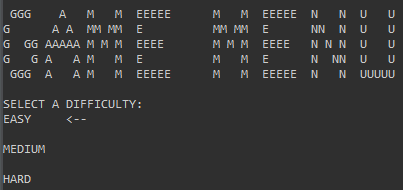
\includegraphics[width=1\linewidth]{game_menu.png}
    \caption{Game Menu displayed on the Terminal}
    \label{fig:game_menu}
\end{figure}

\subsubsection{Implementation of the Game Menu}
In order to make sure that the transition between the game menu and the actual game is done correctly, the OS task responsible for the game behavior and display is suspended as soon as the program is launched. The game menu task is set to high priority and will then be launched. A mutex is used to lock the resources used to read the accelerometer and process the board's tilt to avoid the other threads using them simultaneously. 

The difficulty of the game is set based on the position of the game menu arrow. If the arrow is at position 0, the difficulty is easy. If the arrow is at position 1, the difficulty is medium and if the arrow is at position 2, the difficulty is hard. It also sets where the arrow should be displayed in the menu. The difficulty level of the game determines how many obstacles will be generated.

When the player is ready to play and presses the start button, the game parameters such as the position of the car and the state of the game board are reset, the game difficulty is set, and the task in charge of the game behavior is resumed. This allows the game to start in its initial state. The game menu task is also suspended. It will only be resumed once the player loses or wins the game.

\subsection{Obstacle Generation}  
Obstacle generation plays a key role in making the game engaging and challenging. Obstacles are placed on the road based on the difficulty level and the player’s progress. The generation algorithm ensures:  
\begin{itemize}  
    \item \textbf{Obstacle Placement:} Obstacles are always positioned within the road boundaries to ensure they are reachable by the car.  
    \item \textbf{Randomized Positions:} The row indices for obstacles are determined using a pseudo-random number generator, which provides unpredictable placement. For example, the function \texttt{getRandomNumber0to6()} generates random numbers between 0 and 6, corresponding to possible rows.  
    \item \textbf{Spacing and No Overlap:} Obstacles are spaced apart to ensure they do not overlap, leaving clear paths for the car to navigate.  
    \item \textbf{Dynamic Movement:} Obstacles move leftward on the game board during each game loop iteration, creating the illusion of forward motion.  
\end{itemize}  

For easy difficulty, a single obstacle is generated at a time. For medium difficulty, two obstacles are created, while for hard difficulty, three obstacles are generated simultaneously. The algorithm ensures that each obstacle is placed in a unique row, and all obstacles are initialized at the far-right column of the board.

\subsection{Collision Detection}  
Collision detection is essential to determine if the car hits an obstacle. This is achieved by comparing the car's position with the positions of all obstacles within the same row.  

\begin{itemize}  
    \item \textbf{Car Position:} The car spans four columns, starting from its leading edge. Its position is updated dynamically based on player input.  
    \item \textbf{Obstacle Position:} Obstacles are tracked as they move leftward, and their positions are updated during each loop iteration.  
    \item \textbf{Collision Condition:} A collision occurs if the car and an obstacle share the same row and any part of the car overlaps with the obstacle.  
    \item \textbf{Collision Handling:}  
        \begin{itemize}  
            \item If a collision is detected, a "Game Over" message is displayed, and the game terminates.  
            \item Auditory feedback is generated using the DAC to alert the player.  
        \end{itemize}  
\end{itemize}  

\subsubsection*{Mathematical Representation of Collision Detection}  
Let the car's position on the board be \((x_c, y_c)\), where \(x_c\) represents the row, and \(y_c\) the column of the car's leading edge. Obstacles are represented similarly, with positions \((x_o, y_o)\). A collision is mathematically defined as:  
\begin{equation}  
\text{Collision: } (x_c = x_o) \land (y_c = y_o)  
\end{equation}  

To account for the width of the car, which spans four columns, the collision condition is extended to:  
\begin{equation}  
(x_c = x_o) \land \big(y_o \in \{y_c, y_c + 1, y_c + 2, y_c + 3\}\big)  
\end{equation} 

\subsection{Dynamic Board Updates}  
The game board is updated in each iteration of the game loop to reflect the current state:  

\begin{itemize}  
    \item \textbf{Obstacle Updates:} Obstacles are cleared from their previous positions and shifted leftward. If an obstacle reaches the left edge, it is removed.  
    \item \textbf{Car Placement:} The car's position is updated based on player input and displayed using the string "o/=\o".  
    \item \textbf{Collision Detection During Updates:} If an obstacle moves into a position occupied by the car, a collision is detected, triggering game-over logic.  
    \item \textbf{Board Visualization:} The updated board is displayed after each iteration, showing obstacles, the car, and road boundaries.  
\end{itemize}  

These mechanisms work together to provide a balanced gameplay experience, combining randomness for unpredictability and fairness for skill-based navigation.  


\subsection{Boundary Enforcement}
To ensure that the car remains within the road boundaries, the system constantly checks its position against the road limits. The road boundaries are defined as the minimum and maximum permissible $x$-coordinates:
\begin{equation}
x_{\text{min}} \leq x_c \leq x_{\text{max}}
\end{equation}
If the car attempts to move beyond these boundaries, the movement is restricted, and a warning sound is played to notify the player.

\subsection{Finish Line Detection}
The finish line is positioned at the end of the road and serves as the game's endpoint. When the car reaches the finish line's $y$-coordinate:
\begin{equation}
y_c = y_{\text{finish}}
\end{equation}
a victory message is displayed on the terminal, and a celebratory sound is generated through the speaker. This marks the successful completion of the game.

\section{Conclusion}
This project demonstrates a range of microcontroller capabilities through an interactive car game. The ambitious features, particularly tilt control, showcase advanced interfacing, mathematical processing, and intuitive user interaction. The combination of UART communication, auditory feedback, and multitasking through an operating system further highlights the project’s complexity and innovation. The code is structured and well-documented to ensure readability and maintainability.

\end{document}
